\documentclass{article}

% if you need to pass options to natbib, use, e.g.:
%     \PassOptionsToPackage{numbers, compress}{natbib}
% before loading neurips_2019

% ready for submission
% \usepackage{neurips_2019}

% to compile a preprint version, e.g., for submission to arXiv, add add the
% [preprint] option:
%     \usepackage[preprint]{neurips_2019}

% to compile a camera-ready version, add the [final] option, e.g.:
%     \usepackage[final]{neurips_2019}

%\PassOptionsToPackage{numbers}{natbib}
\usepackage{neurips_2019}

% to avoid loading the natbib package, add option nonatbib:
%     \usepackage[nonatbib]{neurips_2019}

\usepackage[utf8]{inputenc} % allow utf-8 input
\usepackage[T1]{fontenc}    % use 8-bit T1 fonts
\usepackage{hyperref}       % hyperlinks
\usepackage{url}            % simple URL typesetting
\usepackage{booktabs}       % professional-quality tables
\usepackage{amsfonts}       % blackboard math symbols
\usepackage{nicefrac}       % compact symbols for 1/2, etc.
\usepackage{microtype}      % microtypography

\usepackage{microtype}
\usepackage{graphicx}
\usepackage{float}
\usepackage[export]{adjustbox}
\usepackage{subcaption}
\usepackage{booktabs}
\usepackage{xcolor}
\usepackage{xr-hyper}
\usepackage{hyperref}
\usepackage[reqno]{amsmath}
\usepackage{amsfonts, amsthm, amssymb}
\usepackage{algorithm}
\usepackage{algorithmic}
\usepackage[parfill]{parskip}
\usepackage{enumerate}
\usepackage[shortlabels]{enumitem}
\usepackage{bm}
\usepackage{mathtools}

%%%%%% Begin Alden
\DeclarePairedDelimiter\abs{\lvert}{\rvert}

\newcommand{\diam}{\rho}
\newcommand{\set}[1]{\left\{#1\right\}}
\newcommand{\defeq}{\overset{\mathrm{def}}{=}}
\newcommand{\vol}{\mathrm{vol}}
\newcommand{\cut}{\mathrm{cut}}
% \newcommand{\abs}[1]{\left \lvert #1 \right \rvert}
\newcommand{\N}{\mathbb{N}}
\newcommand{\Reals}{\mathbb{R}}
\newcommand{\Rd}{\Reals^d}
\newcommand{\norm}[1]{\left\lVert#1\right\rVert}
\newcommand{\1}{\mathbf{1}}
\newcommand{\Phibf}{\Phi_{u}}
\newcommand{\Psibf}{\Psi_{u}}
\newcommand{\taubf}{\tau_{u}}
\newcommand{\dist}{\mathrm{dist}}

%%% Vectors
\newcommand{\pbf}{p}        % removed bold font
\newcommand{\qbf}{\mathbf{q}}
\newcommand{\ebf}[1]{{e}_{#1}}
\newcommand{\pibf}{\bm{\pi}}

%%% Matrices (no bold font)
\newcommand{\Abf}{A}
\newcommand{\Xbf}{X}             % removed bold font 
\newcommand{\Wbf}{W}
\newcommand{\Lbf}{L}
\newcommand{\Dbf}{D}
\newcommand{\Ibf}[1]{I_{#1}}

%%% Probability distributions (and related items)
\newcommand{\Pbb}{\mathbb{P}}
\newcommand{\Cbb}{\mathbb{C}}
\newcommand{\Ebb}{\mathbb{E}}

%%% Sets
\newcommand{\Cset}{\mathcal{C}}
\newcommand{\Aset}{\mathcal{A}}
\newcommand{\Asig}{\Aset_{\sigma}}
\newcommand{\Csig}{\Cset_{\sigma}}
\newcommand{\Sset}{\mathcal{S}}

%%% Graph quantities
\newcommand{\Cest}{\widehat{C}}

%%% Operators
\DeclareMathOperator*{\argmin}{arg\,min}

%%% Algorithm notation
\newcommand{\ppr}{{\sc PPR}}
\newcommand{\pprspace}{{\sc PPR~}}

\newtheoremstyle{aldenthm}
{6pt} % Space above
{6pt} % Space below
{\itshape} % Body font
{} % Indent amount
{\bfseries} % Theorem head font
{.} % Punctuation after theorem head
{.5em} % Space after theorem head
{} % Theorem head spec (can be left empty, meaning `normal')

\theoremstyle{aldenthm}
\newtheorem{theorem}{Theorem}
\newtheorem{definition}{Definition}
\newtheorem{lemma}{Lemma}
\newtheorem{corollary}{Corollary}

\newtheoremstyle{aldenrmrk}
{6pt} % Space above
{6pt} % Space below
{} % Body font
{} % Indent amount
{\itshape} % Theorem head font
{.} % Punctuation after theorem head
{.5em} % Space after theorem head
{} % Theorem head spec (can be left empty, meaning `normal')

\theoremstyle{aldenrmrk}
\newtheorem{remark}{Remark}
%%%%%% End Alden

\title{Local Spectral Clustering of Density Upper Level Sets}

% The \author macro works with any number of authors. There are two commands
% used to separate the names and addresses of multiple authors: \And and \AND.
%
% Using \And between authors leaves it to LaTeX to determine where to break the
% lines. Using \AND forces a line break at that point. So, if LaTeX puts 3 of 4
% authors names on the first line, and the last on the second line, try using
% \AND instead of \And before the third author name.

\author{%
  David S.~Hippocampus\thanks{Use footnote for providing further information
    about author (webpage, alternative address)---\emph{not} for acknowledging
    funding agencies.} \\
  Department of Computer Science\\
  Cranberry-Lemon University\\
  Pittsburgh, PA 15213 \\
  \texttt{hippo@cs.cranberry-lemon.edu} \\
  % examples of more authors
  % \And
  % Coauthor \\
  % Affiliation \\
  % Address \\
  % \texttt{email} \\
  % \AND
  % Coauthor \\
  % Affiliation \\
  % Address \\
  % \texttt{email} \\
  % \And
  % Coauthor \\
  % Affiliation \\
  % Address \\
  % \texttt{email} \\
  % \And
  % Coauthor \\
  % Affiliation \\
  % Address \\
  % \texttt{email} \\
}

\begin{document}
\maketitle

\begin{abstract}
We analyze Personalized PageRank (PPR), a local spectral method for clustering,
which extract clusters using locally-biased random walks around a user-specified
seed node.  In constrast to pervious work, we adopt a traditional statistical
learning setup, where we obtain samples from an unknown distribution, and aim to
identify connected regions of high-density (density clusters).  We prove that
PPR, run on a neighborhood graph, extracts sufficiently salient density
clusters. We also provide empirical support for our theory.
\end{abstract}

\section{Introduction}
\label{sec: introduction}

In this paper, we study the problem of clustering: splitting a given data set
into groups that satisfy some notion of within-group similarity and
between-group difference.  We focus on spectral clustering, a family of powerful
nonparametric clustering algorithms.  Generally speaking, a spectral algorithm
first constructs a geometric graph $G$, where vertices correspond to samples,
and edges correspond to proximities between samples. It then learns a feature
embedding based on the Laplacian of $G$, and applies a simple clustering
technique (like k-means clustering) in the embedded feature space.

When applied to geometric graphs built from a large number of samples,
global spectral clustering methods can be computationally cumbersome and   
insensitive to the local geometry of the underlying distribution
\citep{leskovec2010,mahoney2012}.  This has led to increased interest in
local spectral clustering algorithms, which leverage locally-biased spectra
computed using random walks around some user-specified seed node.  A popular 
local clustering algorithm is Personalized PageRank (PPR), first introduced by 
\citet{haveliwala2003}, then further developed by
\citep{spielman2011,spielman2014,andersen2006,mahoney2012,zhu2013},
among others.  

Local spectral clustering techniques have been practically very successful
\citep{leskovec2010,andersen2012,gleich2012,mahoney2012,wu2012}, leading 
many authors to develop supporting theory
\citep{spielman2013,andersen2009,gharan2012,zhu2013} that gives worst-case
guarantees on traditional graph-theoretic notions of cluster quality (such as
conductance).  In this paper, we adopt a more traditional statistical viewpoint,
and examine what the output of local clustering on a data set reveals about the
underlying density $f$.  In particular, we examine the ability of PPR to recover
\emph{density clusters} of $f$, defined as the connected components of
the upper level set $\{x \in \Rd : f(x) \geq \lambda\}$ for some $\lambda > 0$
(a central object of interest in the statistical clustering literature, dating
back to \citet{hartigan1981}).   

\paragraph{PPR on a neighborhood graph.} We now describe the clustering
algorithm that will be our focus for the rest of the paper. Let $\Xbf = \{x_1,
\ldots, x_n\}$ be a sample drawn i.i.d.\ from a distribution $\Pbb$ on $\Rd$,
with density $f$.  For a radius $r > 0$, we define $G_{n,r}=(V,E)$ to be the
\emph{$r$-neighborhood graph} of $\Xbf$, an unweighted, undirected graph with
vertices $V=\Xbf$, and an edge $(x_i,x_j) \in E$ if and only if $\norm{x_i -
x_j} \leq r$, where $\norm{\cdot}$ is the $\ell_2$ norm. We denote by $\Abf \in
\Reals^{n \times n}$ the adjacency matrix, with entries $\Abf_{uv} = 1$ if
$(u,v) \in E$ and $0$ otherwise.  We also denote by $\Dbf$ the diagonal degree
matrix, with $\Dbf_{uu} = \sum_{v \in V} \Abf_{uv}$, and by $\Ibf{}$ the $n
\times n$ identity matrix.

Next, we define the PPR vector $\pbf = \pbf(v,\alpha;G_{n,r})$, based on
a seed node $v \in V$ and a teleportation parameter $\alpha \in [0,1]$, to be 
the solution of the following linear system:
\begin{equation}
\label{eqn: ppr_vector}
\pbf = \alpha \ebf{v} + (1 - \alpha) \pbf \Wbf,
\end{equation}
where $\Wbf = (\Ibf{} + \Dbf^{-1}\Abf)/2$ is the lazy random walk matrix over
$G_{n,r}$ and $e_{v}$ is the indicator vector for node $v$ (that has a 1 in the
$v$th position and 0 elsewhere). For a level $\beta > 0$ and a target volume
$\vol_0 > 0$, we define a \emph{$\beta$-sweep cut} of $\pbf = (p_u)_{u \in V}$
as   
\begin{equation}
\label{eqn: sweep_cuts}
S_\beta := \set{u \in V: \frac{p_u}{\Dbf_{uu}} > \frac{\beta}{\vol_{0}}}.
\end{equation}
We will use the normalized cut metric to determine which sweep cut $S_{\beta}$
is the best cluster estimate. For a set $S \subseteq V$ with complement $S^c = V
\setminus S$, we define \smash{$\cut(S;G_{n,r}) := \sum_{u \in S, v \in S^c}
\Abf_{uv}$}, and \smash{$\vol(S; G_{n,r}) := \sum_{u \in S} \Dbf_{uu}$}.  We
define the \emph{normalized cut} of $S$ as
\begin{equation}
\label{eqn: normalized_cut}
\Phi(S; G_{n,r}) := \frac{\cut(S;G_{n,r})}{\min \set{\vol(S; G_{n,r}), \vol(S^c; G_{n,r})}}.
\end{equation}
Having computed sweep cuts $S_{\beta}$ over a range \smash{$\beta \in  
(\frac{1}{40},\frac{1}{11})$}\footnote{The choice of a specific range such as  
\smash{$(\frac{1}{40}, \frac{1}{11})$} is standard in the analysis of PPR
algorithms, see, e.g., \citep{zhu2013}.}, we output the cluster estimate
\smash{$\Cest = S_{\beta^*}$} that has minimum normalized cut.
%\smash{$\Phi(S_{\beta^*}; G_{n,r})$}. 
For concreteness, this is summarized in Algorithm \ref{alg: ppr}. 

\begin{algorithm}
\caption{PPR on a neighborhood graph}
\label{alg: ppr}	
{\bfseries Input:} data $\Xbf=\{x_1,\ldots,x_n\}$, radius $r > 0$, teleportation
parameter $\alpha \in [0,1]$, seed $v \in \Xbf$, target stationary volume
$\vol_0 > 0$. \\     
{\bfseries Output:} cluster $\Cest \subseteq V$.
\begin{algorithmic}[1]
  \STATE Form the neighborhood graph $G_{n,r}$.
  \STATE Compute the PPR vector $p=\pbf(v, \alpha; G_{n,r})$ as in \eqref{eqn: 
    ppr_vector}. 
  \STATE For \smash{$\beta \in (\frac{1}{40}, \frac{1}{11})$} compute sweep cuts 
  $S_{\beta}$ as in \eqref{eqn: sweep_cuts}.
  \STATE Return as a cluster \smash{$\Cest = S_{\beta^*}$}, where  
  $$
  \beta^* = \argmin_{\beta \in (\frac{1}{40}, \frac{1}{11})} \Phi(S_{\beta}; G_{n,r}).
  $$
\end{algorithmic}
\end{algorithm}

\paragraph{Estimation of density clusters.} Let \smash{$\Cbb_f(\lambda)$} denote 
the connected components of the density upper level set $\{x \in \Rd: f(x) >
\lambda\}$.  For a given density cluster \smash{$\Cset \in \Cbb_f(\lambda)$}, we
call $\Cset[\Xbf] = \Cset \cap \Xbf$ the \emph{empirical density cluster}. The
size of the symmetric set difference between estimated and empirical clusters is 
a commonly used metric to quantify cluster estimation error
\citep{korostelev1993,polonik1995,rigollet2009}.  

\begin{definition}[Symmetric set difference]
  \label{def: symmetric_set_diff}
  For an estimator \smash{$\Cest \subseteq \Xbf$} and set
  $\mathcal{S} \subseteq \Reals^d$, we define   
  \begin{equation}
    \label{eqn: misclassification_rate}
    \Delta(\Cest, \mathcal{S}) := \abs{\Cest \setminus \mathcal{S}[\Xbf] \cup
      \mathcal{S}[\Xbf] \setminus \Cest},
  \end{equation}
  the cardinality of the symmetric set difference between 
  \smash{$\Cest$} and $\mathcal{S} \cap \Xbf = \mathcal{S}[\Xbf]$. 
\end{definition}

However, the symmetric set difference does not measure whether \smash{$\Cest$} 
can distinguish any two distinct clusters \smash{$\Cset,\Cset' \in
  \Cbb_f(\lambda)$}. We therefore also study a second notion of cluster
estimation, first introduced by \citet{hartigan1981}, and defined
asymptotically. 

\begin{definition}[Consistent density cluster estimation]
  \label{def: consistent_density_cluster_estimation}
  For an estimator \smash{$\Cest \subseteq \Xbf$} and cluster 
  \smash{$\Cset \in \Cbb_f(\lambda)$}, we say \smash{$\Cest$} is a consistent 
  estimator of $\Cset$ if for all \smash{$\Cset' \in \Cbb_f(\lambda)$} with
  $\Cset \not= \Cset'$, the following holds as $n \to \infty$: 
  \begin{equation}
    \label{eqn: consistent_density_cluster_recovery}
    \Cset[\Xbf] \subseteq \Cest \quad \text{and} \quad
    \Cest \cap \Cset'[\Xbf] = \emptyset,
  \end{equation}
  with probability tending to 1.
\end{definition}

\paragraph{Summary of results.} A summary of our results (and outline for this
paper) is as follows.

\begin{enumerate}
\item In Section \ref{sec: consistent_cluster_estimation_with_ppr}, we introduce
  a set of natural geometric conditions on the density cluster $\Cset$
  %formalize a measure of difficulty based on these geometric conditions, 
  and show that when Algorithm \ref{alg: ppr} is properly initialized, the size of
  the symmetric set difference of \smash{$\Cest$} and a thickened version of the
  density cluster $\Csig$ can be bounded in a meaningful way.
  % this difficulty measure.  
	
\item We further show in Section \ref{sec:
    consistent_cluster_estimation_with_ppr} that if the density cluster 
  $\Cset$ is particularly well-conditioned, Algorithm \ref{alg: ppr}
  will consistently estimate a density cluster in the sense of
  \eqref{eqn: consistent_density_cluster_recovery}. 
	
\item In Section \ref{sec: analysis}, we detail some of the analysis required to
  prove our main results, and expose the parts various geometric quantities play 
  in the difficulty of the clustering problem. 
	
\item In Section \ref{sec: experiments}, we empirically investigate the
  tightness of our analysis, and provide examples showing how violations of our
  geometric conditions impact density cluster recovery by PPR.
\end{enumerate}

Our main takeaway: PPR, run on a neighborhood graph, recovers geometrically
compact high-density clusters. 

\paragraph{Related work.} In addition to the background on local spectral
clustering given previously, a few related lines of work are worth
highlighting. \citep{shi2009,schiebinger2015} examine the consistency of  
spectral algorithms in recovering the latent labels in certain
nonparametric mixture models. Their results focus on global rather than local 
methods, and thus impose global rather than local conditions on the nature
of the density. Moreover, they do not in general guarantee recovery of density 
clusters, which is the focus in our work. Perhaps most importantly, these works
rely on general cluster saliency conditions, which implicitly depend on many
distinct geometric aspects of the cluster $\Cset$ under consideration. We make
this dependence more explicit, and in doing so expose the role each geometric
condition plays in the clustering problem. 

More broadly, density clustering and level set estimation is a well-studied
problem. \citet{polonik1995, rigollet2009} study density clustering under the 
symmetric set difference metric, \citet{tsybakov1997, singh2009} describe
minimax optimal level set estimators under Hausdorff loss and
\citet{hartigan1981, chaudhuri2010} consider consistent estimation of the
cluster tree, to note but a few works. Our goal is not to improve on these
results, nor to offer a better algorithm for level set estimation; indeed, seen as
a density clustering algorithm, PPR has none of the optimality guarantees 
found in the aforementioned works. Instead, our motivation is start with a
widely-used local spectral method, PPR, and to better understand and
characterize the distinctions between those density clusters which are
well-conditioned for PPR, and those which are not. 

\section{Estimation of well-conditioned density clusters}
\label{sec: consistent_cluster_estimation_with_ppr}

We formalize some geometric conditions, and use these to define a condition
number $\kappa(\Cset)$, which measures the difficulty PPR will have in  
estimating $\Cset$. (Our theoretical guarantees for PPR will be framed in terms 
of $\kappa(\Cset)$.)

\paragraph{Geometric conditions on density clusters.} At a high level, for PPR
to be successful, the underlying density cluster must be geometrically
well-conditioned.  At a minimum, we want to avoid sets that contain arbitrarily
thin bridges or spikes.  Hence, as in \citet{chaudhuri2010}, we consider a
thickened version of \smash{$\Cset \in \Cbb_f(\lambda)$} defined as 
$\Csig := \set{x \in \Reals^d: \dist(x,\Cset) \leq \sigma}$, which 
we call the \emph{$\sigma$-expansion} of $\Cset$. Here 
\smash{$\dist(x,\Cset) := \inf_{y \in \Cset} \norm{y - x}$}.  We now list our
conditions on $\Csig$.

\begin{enumerate}[label=(A\arabic*)]
\item
  \label{asmp: bounded_density}
  \emph{Bounded density within cluster:} There exist constants
  $0<\lambda_{\sigma}< \Lambda_{\sigma}<\infty$ such that 
  $\lambda_{\sigma} \leq \inf_{x \in \Csig} f(x) \leq \sup_{x \in \Csig} f(x)
  \leq \Lambda_{\sigma}$. 
  
\item
  \label{asmp: cluster_separation}
  \emph{Cluster separation:}
  For all clusters $\Cset' \in \Cbb_f(\lambda)$ with $\Cset' \not= \Cset$, 
  $\dist(\Csig,\Csig') > \sigma$, where $\dist(\Csig,\Csig') := \inf_{x
    \in \Csig} \dist(x,\Csig')$.  
    
\item 
  \label{asmp: low_noise_density}
  \emph{Low noise density:} There exist $\gamma,c_0 > 0$ such that for 
  $x \in \Rd$ with $0 < \dist(x, \Csig) \leq \sigma$,   
  $\inf_{x' \in \Csig} f(x') - f(x) \geq  c_0 \dist(x, \Csig)^{\gamma}$.
	
  %%% AJG 5/20: Should I turn this into two conditions?
\item
  \label{asmp: embedding}
  \emph{Lipschitz embedding:}
  There exists $g: \Reals^d \to \Reals^d$ with the following properties: i)
  we have $\Csig = g(\mathcal{K})$, for a convex set $\mathcal{K} \subseteq \Rd$
  with $\mathrm{diam}(\mathcal{K}) = \sup_{x,y \in \mathcal{K}}\norm{x - y} =:
  \diam < \infty$; ii) $\det(\nabla g (x)) = 1$ for all $x \in \Csig$, where
  $\nabla g(x)$ is the Jacobian of $g$ evaluated at $x$; and iii) for some $L
  \geq 1$,   
  \begin{equation*}
    \frac{1}{L}\norm{x - y} \leq \norm{g(x) - g(y)} \leq L \norm{x - y} ~
    \text{for all $x,y \in \mathcal{K}$}. 
  \end{equation*}
  Succintly, $\Csig$ is the image of a convex set with finite diameter 
  under a  measure preserving, bi-Lipschitz transformation. 

\item
  \label{asmp: bounded_volume}
  \emph{Bounded volume:}
  Let the neighborhood graph radius $0 < r \leq \sigma/2d$ be such that
  \begin{equation*}
    2 \int_{\Csig} \Pbb(B(x,r)) f(x) dx \leq \int_{\Rd} \Pbb(B(x,r)) f(x) dx,
  \end{equation*}
  where $B(x,r)$ is the closed ball of radius $r$ at $x$.
\end{enumerate}

To motivate these conditions, \citet{zhu2013} show for arbitrary graph $G =
(V,E)$ and subset of vertices $S \subseteq V$, the PPR estimate \smash{$\Cest$}
of subset $S$ satisfies, for a constant $c>0$,
\begin{equation}
\label{eqn: graph_symmetric_set_difference_1}
\vol(\Cest \setminus S; G) + \vol(S \setminus \Cest; G) \leq c \bigl( \Phi(S,G)
\cdot \tau_{\infty}(G[S])\bigr) \vol(S;G),
\end{equation}
where $\Phi(S;G)$ is the normalized cut of $S$ (as defined in \eqref{eqn:
  normalized_cut}), and \smash{$\tau_{\infty}(G[S])$} is called the \emph{mixing
  time} of a random walk over the induced subgraph $G[S]$ (to be defined
precisely later, in \eqref{eqn: mixing_time}).  The left-hand side in
\eqref{eqn:  graph_symmetric_set_difference_1} resembles a (degree-weighted) 
form of the symmetric set difference metric in \eqref{eqn:
  misclassification_rate}.  As we will show in Section \ref{sec:
  analysis}, the conditions \ref{asmp: bounded_density}--\ref{asmp:
  bounded_volume} allow us to upper bound the normalized cut 
\smash{$\Phi(\Csig[\Xbf]; G_{n,r})$}, and the mixing time 
\smash{$\tau_{\infty}(G_{n,r}[\Csig[\Xbf]])$}.  (Informally, 
\ref{asmp: cluster_separation}, \ref{asmp: low_noise_density} yield an upper
bound on \smash{$\cut(\Csig[\Xbf]; G_{n,r})$}, and \ref{asmp: bounded_density}
yields a lower bound on \smash{$\vol(\Csig[\Xbf]; G_{n,r})$}; together with 
\ref{asmp: bounded_volume}, this gives an upper bound on the normalized cut.  On 
the other hand, \ref{asmp: bounded_density}, \ref{asmp: embedding} preclude
bottlenecks in the induced subgraph \smash{$G_{n,r}[\Csig[\Xbf]]$}, and combined
with \ref{asmp: embedding}, this leads to an upper bound on the mixing time over 
this subgraph.) 

\paragraph{Condition number.} Motivated by \eqref{eqn:
  graph_symmetric_set_difference_1}, we will define $\kappa(\Cset)$ to be an
upper bound on the product \smash{$\Phi(\Csig[\Xbf]; G_{n,r}) \cdot
  \tau_{\infty}(G_{n,r}[\Csig[\Xbf]])$}. The smaller $\kappa(\Cset)$ is, the
more success PPR will have in recovering $\Cset$. Let $\theta := (r, \sigma,
\lambda, \lambda_{\sigma}, \Lambda_{\sigma}, \gamma, \diam, L)$ contain the
geometric parameters from \ref{asmp:  bounded_density}--\ref{asmp:
  bounded_volume}.  

\begin{definition}[Well-conditioned density clusters]
  For $\lambda > 0$ and \smash{$\Cset \in \Cbb_f(\lambda)$}, let $\Cset$ satisfy 
  \ref{asmp: bounded_density}--\ref{asmp: bounded_volume} for some
  $\theta$. Then, for universal constants $c_1, c_2, c_3 > 0$ to be specified
  later, we set 
  \begin{equation}
    \label{eqn: condition_number_1}
    \Phibf(\theta) 
    := c_1 r \frac{d}{\sigma} \frac{\lambda}{\lambda_{\sigma}}
    \frac{(\lambda_{\sigma} - c_0 \frac{r^{\gamma}}{\gamma +
        1})}{\lambda_{\sigma}},~  
    \taubf(\theta) := c_2 \frac{\Lambda_{\sigma}^4 d^3 \rho^2
      L^2}{\lambda_{\sigma}^4 r^2} \log^2\left(\frac{1}{r}\right) + c_3,
  \end{equation}
  and letting \smash{$\kappa(\Cset) := \Phi_{u}(\theta) \cdot
    \tau_{u}(\theta)$}, we call $\Cset$ a 
  \emph{$\kappa$-well-conditioned density cluster}.  
\end{definition}

We note that $\Phibf(\theta)$ and $\taubf(\theta)$ are exactly the upper bounds 
on \smash{$\Phi(\Csig[\Xbf]; G_{n,r})$} and
\smash{$\tau_{\infty}(G_{n,r}[\Csig[\Xbf]])$} that we derive in our analysis
later, in Section \ref{sec: analysis}. 

\paragraph{Well-initialized algorithm.} As is typical in the local clustering
literature, our algorithmic results will be stated with respect to specific
ranges of each of the user-specified parameters. In particular, for a
well-conditioned density cluster $\Cset$ (with respect to some $\theta$), we
require 
\begin{equation}
\begin{gathered}
\label{eqn: initialization}
0 < r \leq \frac{\sigma}{2d}, \quad 
\alpha \in [1/10, 1/9] \cdot \frac{1}{\taubf(\theta)}, \\
v \in \Csig[\Xbf]^g, \quad
\vol_0 \in [3/4,5/4] \cdot n(n-1) \int_{\Csig} \Pbb(B(x,r)) f(x) dx, 
\end{gathered}
\end{equation}
where \smash{$\Csig[\Xbf]^g \subseteq \Csig[\Xbf]$} will be some large
(``good'') subset of $\Csig[\Xbf]$. In particular, abbreviating $\vol_{n,r}(S)
:= \vol(S; G_{n,r})$ for $S \subseteq \Xbf$, we will have
\smash{$\vol_{n,r}(\Csig[\Xbf]^g) \geq \vol_{n,r}(\Csig[\Xbf])/2$}.  

\begin{definition}
If the input parameters to Algorithm \ref{alg: ppr} satisfy \eqref{eqn:
  initialization} for some well-conditioned density cluster $\Cset$, we
say the algorithm is \emph{well-initialized}. 
\end{definition}

In practice it is clearly not feasible to set hyperparameters based on the
underlying (unknown) density $f$. Typically, one tunes PPR over a range of
hyperparameters and optimizes for some criterion such as minimum normalized cut;
it is not obvious how this scheme would affect the performance of PPR in the
density clustering context.  

\paragraph{Main theorems.} The results of Section \ref{sec: analysis}, combined 
with \eqref{eqn: graph_symmetric_set_difference_1}, give an upper bound on the
volume of \smash{$\Cest \setminus \Csig[\Xbf]$} and \smash{$\Csig[\Xbf]
  \setminus \Cest$},  
\begin{equation}
\label{eqn: graph_symmetric_set_difference}
\vol_{n,r}(\Cest \setminus \Csig[\Xbf]) + \vol_{n,r}(\Csig[\Xbf] \setminus
\Cest) \leq c \kappa(\Cset) \vol_{n,r}(\Csig[\Xbf]). 
\end{equation}
To translate \eqref{eqn: graph_symmetric_set_difference} into meaningful bounds
on the symmetric set difference metric \smash{$\Delta(\Csig[\Xbf], \Cest)$}, we
want to preclude vertices $x \in \Xbf$ from having arbitrarily small degree, and
so we make some regularity assumptions on $\mathcal{X} := \mathrm{supp}(f)$. Let
$\nu$ denote the Lebesgue measure on $\Rd$, and $\nu_d := \nu(B)$ be the measure
of the unit ball $B = B(0,1)$. 
\begin{enumerate}[label=(A\arabic*)]
  \setcounter{enumi}{5}
\item 
  \label{asmp: valid_region}
  \emph{Regular support:} There exists some constant $\lambda_{\min} > 0$ such 
  that $\lambda_{\min} < f(x)$ for all $x \in \mathcal{X}$. Additionally, there
  exists some $c > 0$ such that for each $x \in \partial \mathcal{X}$,
  $\nu(B(x,r) \cap \mathcal{X}) \geq c \nu_d r^d$. 
\end{enumerate}
Note that the latter condition in \ref{asmp: valid_region} will hold if the
boundary $\partial \mathcal{X}$ is sufficiently regular.  Now we present our
main bound on the symmetric set difference metric.

\begin{theorem}
  \label{thm: misclassification_rate}
  Fix $\lambda > 0$, let \smash{$\Cset \in \Cbb_f(\lambda)$} be a
  $\kappa$-well-conditioned density cluster (with respect to some $\theta$), and
  additionally assume $f$ satisfies \ref{asmp: valid_region}. If Algorithm
  \ref{alg: ppr} is well-initialized, there exists a universal constant $c >
  0$ such that with probability tending to 1 as $n \to \infty$,  
  \begin{equation}
    \label{eqn: misclassification_rate_ub}
    \Delta(\Csig[\Xbf], \Cest) \leq c \kappa(\Cset)
    \frac{\Lambda_{\sigma}}{\lambda_{\min}}. 
  \end{equation}
\end{theorem}

The proof of Theorem \ref{thm: misclassification_rate}, along with all other
proofs in this paper, is deferred to the supplementary material. Note that this 
result says the symmetric set difference metric \smash{$\Delta(\Csig[\Xbf],
  \Cest)$} is proportional to the difficulty of the clustering problem, as
measured by the condition number $\kappa(\Cset)$. 

Neither \eqref{eqn: graph_symmetric_set_difference} nor \eqref{eqn:
  misclassification_rate_ub} imply consistent density cluster estimation in the 
sense of \eqref{eqn: consistent_density_cluster_recovery}. This notion of
consistency requires a uniform bound over $\pbf$: for all \smash{$\Cset'
  \in \Cbb_f(\lambda), \Cset' \neq \Cset$}, and each $u \in \Cset, w \in
\Cset'$,  
\begin{equation}
\label{eqn: ppr_gap}
\frac{p_{w}}{\Dbf_{ww}} \leq \frac{1}{40\vol_0} < \frac{1}{11\vol_0} \leq
\frac{p_u}{\Dbf_{uu}}, 
\end{equation}
so that any sweep cut $S_{\beta}$ for $\beta \vol_0 \in [1/40,1/11]$ (i.e., any
sweep cut considered by Algorithm \ref{alg: ppr}) will fulfill both conditions
laid out in \eqref{eqn: consistent_density_cluster_recovery}. In Theorem
\ref{thm: consistent_recovery_of_density_clusters}, we show that a sufficiently
small upper bound on $\kappa(\Cset)$ ensures such a gap exists with probability
1 as $n \to \infty$, and hence guarantees \smash{$\Cest$} will be a consistent  
estimator. As was the case before, we wish to preclude arbitrarily low degree
vertices, this time for points $x \in \Cset'[\Xbf]$. 
\begin{enumerate}[label=(A\arabic*)]
  \setcounter{enumi}{6}
\item 
  \label{asmp: C'_bounded_density}
  \emph{Bounded density in other clusters:} Letting $\sigma,\lambda_{\sigma}$ be 
  as in \ref{asmp: bounded_density}, for each $\Cset' \in \Cbb_f(\lambda)$ and
  for all $x \in \Csig'$, $\lambda_{\sigma} \leq f(x)$. 
\end{enumerate}

Next we give our main result on consistent cluster recovery by PPR.

\begin{theorem}
  \label{thm: consistent_recovery_of_density_clusters}
  Fix $\lambda > 0$, let $\Cset \in \Cbb_f(\lambda)$ be a
  $\kappa$-well-conditioned density cluster (with respect to some $\theta$), and
  additionally assume $f$ satisfies \ref{asmp: C'_bounded_density}. If Algorithm
  \ref{alg: ppr} is well-initialized, there exists a universal constant $c >  0$
  such that if  
  \begin{equation}
    \label{eqn: kappa_ub}
    \kappa(\Cset) \leq c \frac{\lambda_{\sigma}^2r^d
      \nu_d}{\Lambda_{\sigma}\Pbb(\Csig)}, 
  \end{equation}
  then the output set $\Cest \subseteq \Xbf$ is a consistent estimator for
  $\Cset$, in the sense of Definition \ref{def: consistent_density_cluster_estimation}. 
\end{theorem}

\begin{remark}
  We note that the restriction on $\kappa(\Cset)$ imposed by \eqref{eqn:
    kappa_ub} results in a symmetric set difference \smash{$\Delta(\Csig[\Xbf],
    \Cest)$} on the order of $r^d$. In plain terms, we are able to recover a
  density cluster $\Cset$ in the sense of \eqref{eqn:
    consistent_density_cluster_recovery} only when we can guarantee a very small
  fraction of points will be misclassified. This strong condition is the price
  we pay in order to obtain the uniform bound of \eqref{eqn: ppr_gap}. 
\end{remark}

\begin{remark}
  While taking the radius of the neighborhood graph $r \to 0$ as $n \to
  \infty$ (thereby ensuring $G_{n,r}$ is sparse) is computationally
  attractive, the presence of a factor of \smash{$\log^2(1/r)/r$} in
  $\kappa(\Cset)$ unfortunately prevents us from making claims about the
  behavior of PPR in this regime. Although the restriction to a kernel
  function fixed in $n$ is standard for spectral clustering theory
  \citep{schiebinger2015,vonluxburg2008}, it is an interesting question whether
  PPR exhibits some degeneracy over $r$-neighborhood graphs as $r \to 0$, or if
  this is merely looseness in our upper bounds.  
\end{remark}

\paragraph{Approximate PPR vector.}  In practice, exactly solving \eqref{eqn:
  ppr_vector} may be too computationally expensive. To address this limitation,
\citet{andersen2006} introduced the \emph{$\epsilon$-approximate} PPR vector
(aPPR), which we will denote by \smash{$\pbf^{(\epsilon)}$}. We refer the
curious reader to \citet{andersen2006} for a formal algorithmic definition of
the aPPR vector, and limit ourselves to highlighting a few salient points: the
aPPR vector can be computed in order $\mathcal{O}(1/(\epsilon\alpha))$ time,
while satisfying the following uniform error bound: 
\begin{equation}
\label{eqn: appr_error}
\textrm{for all $u \in V$}, \quad \pbf(u) - \epsilon \Dbf_{uu}\leq
\pbf^{(\epsilon)}(u) \leq \pbf(u).  
\end{equation}
Application of \eqref{eqn: appr_error} within the proofs of Theorems \ref{thm:
  misclassification_rate} and \ref{thm: consistent_recovery_of_density_clusters}
leads to analogous results which hold for \smash{$\pbf^{(\epsilon)}$}. We
formally state and prove this in the supplement. 

\section{Analysis}
\label{sec: analysis}

The primary technical contribution of our work is showing that the geometric
conditions \ref{asmp: bounded_density}--\ref{asmp: bounded_volume} translate to 
meaningful bounds on the normalized cut and mixing time of $\Csig[\Xbf]$ in
$G_{n,r}$. In doing so, we elaborate on how some of the geometric conditions
introduced in Section \ref{sec: consistent_cluster_estimation_with_ppr}
contribute to the difficulty of the clustering problem. 

\paragraph{Normalized cut.} We start with a finite sample upper bound on the
normalized cut \eqref{eqn: normalized_cut} of $\Cset_\sigma[\Xbf]$. For
simplicity, we write $\Phi_{n,r}(\Csig[\Xbf]) := \Phi(\Csig[\Xbf]; G_{n,r})$. 

\begin{theorem}
  \label{thm: conductance_upper_bound}
  Fix $\lambda > 0$, and assume $\Cset \in \Cbb_f(\lambda)$ satisfies
  Assumptions \ref{asmp: bounded_density}--\ref{asmp: low_noise_density}, 
  \ref{asmp: bounded_volume} for some $r, \sigma, \lambda_{\sigma}, c_0, \gamma
  > 0$ (no bound on maximum density is needed). Then for any $0 < \delta < 1$,
  $\epsilon > 0$, if 
  \begin{equation}
    \label{eqn: conductance_sample_complexity}
    n \geq \frac{(2+\epsilon)^2\log(3/\delta)}{\epsilon^2}\left(\frac{25}
      {6 \lambda_{\sigma}^2\nu(\Csig) \nu_d r^d}\right)^2,
  \end{equation}
  then
  \begin{equation}
    \label{eqn: conductance_additive_error_bound}
    \frac{\Phi_{n,r}(\Csig[\Xbf])}{r} \leq c_1 \frac{d}{\sigma}
    \frac{\lambda}{\lambda_{\sigma}} \frac{(\lambda_{\sigma} -
      c_0\frac{r^{\gamma}}{\gamma+1})}{\lambda_{\sigma}} + \epsilon, 
  \end{equation}
  with probability at least $1-\delta$ (where $c_1 > 0$ is a universal constant).
\end{theorem}

\begin{remark}
  \label{rmk: diameter}
  Observe that the diameter $\rho$ is absent from Theorem \ref{thm:
    conductance_upper_bound}, in contrast to the condition number
  $\kappa(\Cset)$, which worsens (increases) as $\rho$ increases. This
  reflects established wisdom regarding spectral partitioning
  algorithms more generally \citep{guattery1995, hein2010}, albeit newly applied
  to the density clustering setting. It suggests that if the diameter $\rho$ is
  large, PPR may fail to recover $\Csig[\Xbf]$ even when $\Cset$ is
  sufficiently well-conditioned to ensure $\Csig[\Xbf]$ has a small normalized
  cut in $G_{n,r}$. This intuition will be supported by simulations in Section
  \ref{sec: experiments}. 
\end{remark}

\paragraph{Mixing time.} For $S \subseteq V$, denote by $G[S] = (S, E_S)$ the
subgraph induced by $S$ (where the edges are $E_S = E \cap (S \times S)$). Let
$\Wbf_S$ be the (lazy) random walk matrix over $G[S]$, and write  
$$
q_{v}^{(t)}(u) = e_v\Wbf_S^t e_u
$$
for the $t$-step transition probability of the lazy random walk over $G[S]$
originating at $v \in V$. Also write \smash{$\pi = (\pi(u))_{u \in S}$}
for the stationary distribution of this random walk.  (As
$\Wbf_S$ is the transition matrix of a lazy random walk, 
it is well-known that a unique stationary distribution exists and is given by 
\smash{$\pi(u) = (\Dbf_S)_{uu}/\vol(S; G[S])$}, where we write $\Dbf_S$ for the  
degree matrix of $G[S]$.) We define the \emph{mixing time} of $G[S]$ as
\begin{equation}
\label{eqn: mixing_time}
\tau_{\infty}(G[S]) = \min\set{ t: \frac{\pi(u) - q_{v}^{(t)}(u)}
  {\pi(u)} \leq \frac{1}{4}, \; \text{for $u,v \in V$}}. 
\end{equation}
Next, we give an asymptotic (in the number of vertices $n$) upper bound on
$\tau_{\infty}(G_{n,r}[\Csig[\Xbf]])$.  

\begin{theorem}
  \label{thm: mixing_time_upper_bound}
  Fix $\lambda > 0$, and assume that \smash{$\Cset \in \Cbb_f(\lambda)$}
  satisfies Assumptions \ref{asmp: bounded_density} and \ref{asmp: embedding}
  for some $\sigma, \lambda_{\sigma}, \Lambda_{\sigma}, \rho, L > 0$. Then, for
  any \smash{$0 < r < \sigma/2\sqrt{d}$}, with probability 1,
  \begin{equation} 
    \label{eqn: mixing_time_upper_bound}
    \limsup_{n \to \infty}\tau_{\infty}(G_{n,r}[\Csig[\Xbf]]) \leq c_1
    \frac{\Lambda_{\sigma}^4 d^3 \rho^2 L^2}{\lambda_{\sigma}^4 r^2}
    \log^2\left(\frac{1}{r}\right) + c_2,
  \end{equation}
  for $c_1,c_2 > 0$ universal constants. 
\end{theorem}

To the best of our knowledge, Theorem \ref{thm: mixing_time_upper_bound} is the
first bound, albeit asymptotic, on the mixing time of random walks over
neighborhood graphs which is independent of $n$, the number of vertices. 

\begin{remark}
  The embedding assumption \ref{asmp: embedding} and Lipschitz parameter $L$
  play an important role in proving the upper bound of Theorem \ref{thm:
    mixing_time_upper_bound}. There is some interdependence between $L$ and
  $\sigma,\rho$, which might lead one to hope that \ref{asmp: embedding} is
  non-essential. However, it is not possible to eliminate condition \ref{asmp:
    embedding} without incurring an additional factor of at least
  $(\rho/\sigma)^d$ in \eqref{eqn: mixing_time_upper_bound}, achieved, for
  instance, when $\Csig$ is a dumbbell-like set consisting of two balls of
  diameter $\rho$ linked by a cylinder of radius
  $\sigma$. \citet{abbasi-yadkori2016, abbasi-yadkori2016a}  
  develop theory regarding bi-Lipschitz deformations of convex sets, wherein it
  is observed that star-shaped sets as well as half-moon shapes of the type we
  consider in Section \ref{sec: experiments} both satisfy \ref{asmp: embedding}
  for reasonably small values of $L$. 
\end{remark}

\section{Experiments}
\label{sec: experiments}

We provide numerical experiments to investigate the tightness of our bounds on normalized cut and mixing time of $\Csig[\Xbf]$, and examine the performance of \pprspace on the ``two moons'' dataset. For space reasons, we defer details of the experimental settings to the supplement.

\paragraph{Validating theoretical bounds}

\begin{figure}
  \centering
%  \begin{adjustbox}{minipage=\linewidth}
%    \begin{subfigure}{.33\linewidth}
  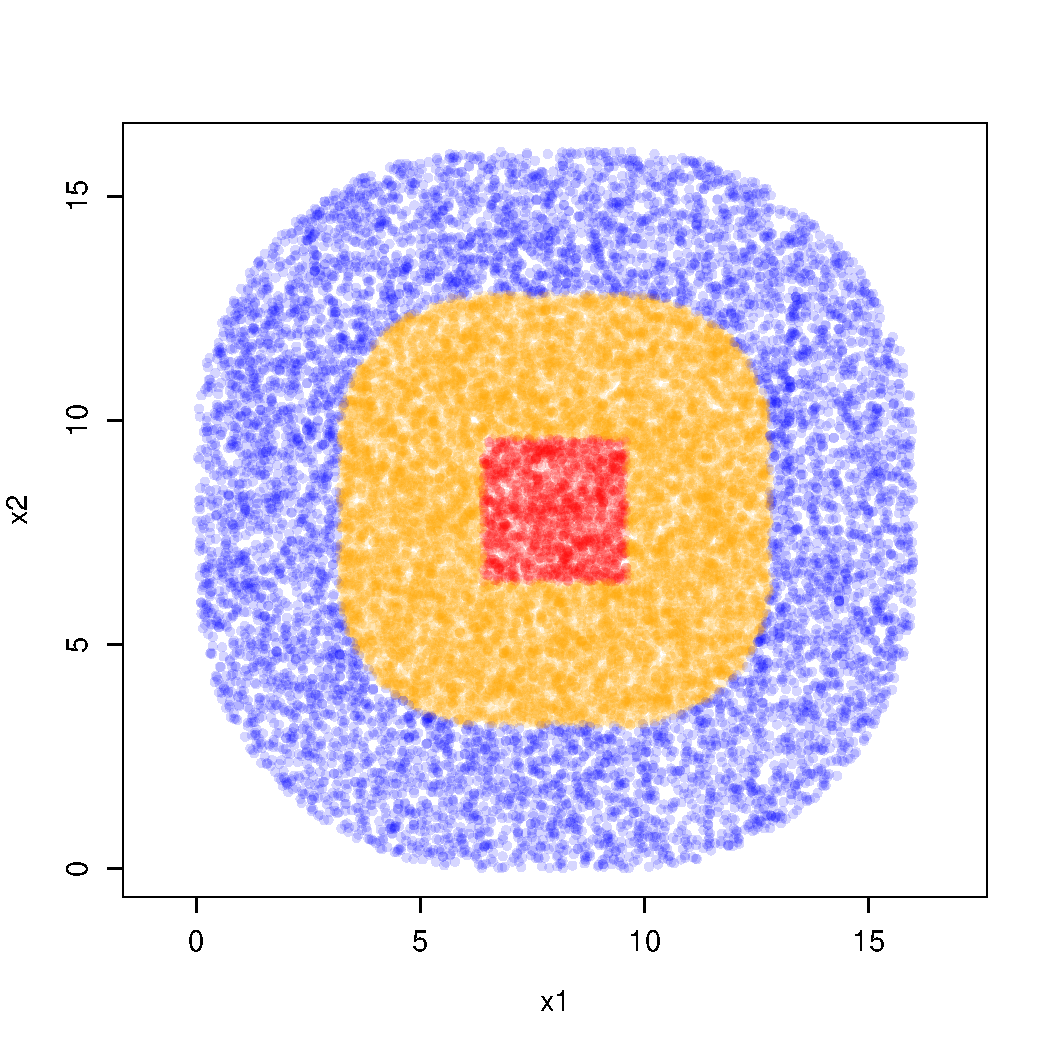
\includegraphics[width=0.33\textwidth]{example1plots/sample2}
%      \caption{}
%    \end{subfigure}
%    \begin{subfigure}{.33\linewidth}
  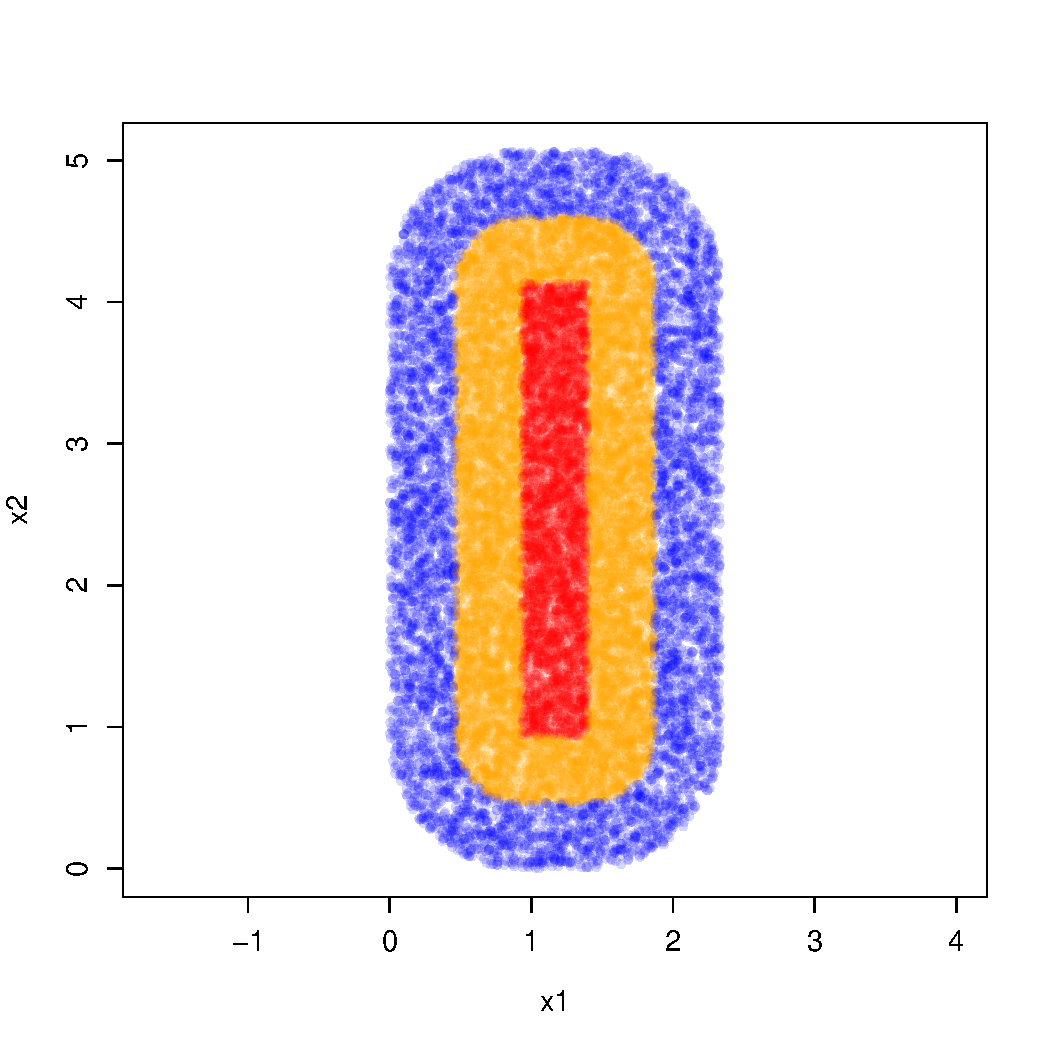
\includegraphics[width=0.33\textwidth]{example1plots/sample1}
%      \caption{}
%    \end{subfigure}
%    \begin{subfigure}{.33\linewidth}
      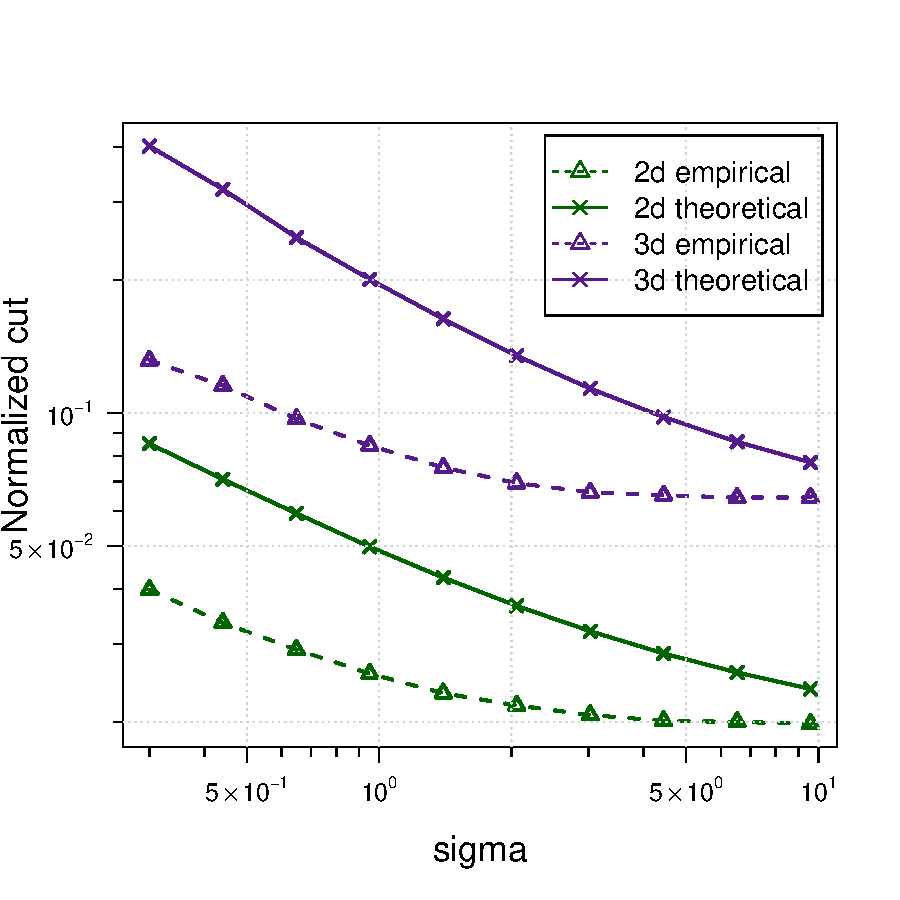
\includegraphics[width=0.33\textwidth]{example1plots/sigma_normalized_cut_plot}
%      \caption{}
%    \end{subfigure}
     
%    \begin{subfigure}{.33\linewidth}
      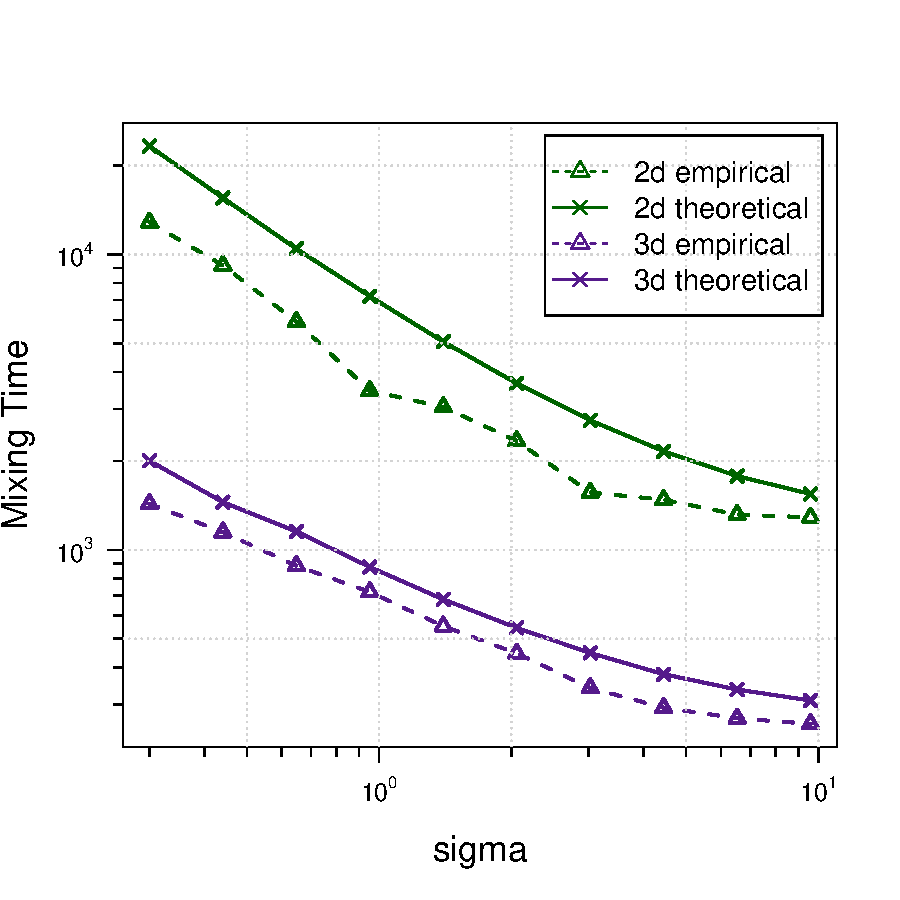
\includegraphics[width=0.33\textwidth]{example1plots/sigma_mixing_time_plot}
%      \caption{}
%    \end{subfigure}
    \begin{subfigure}{.33\linewidth}
      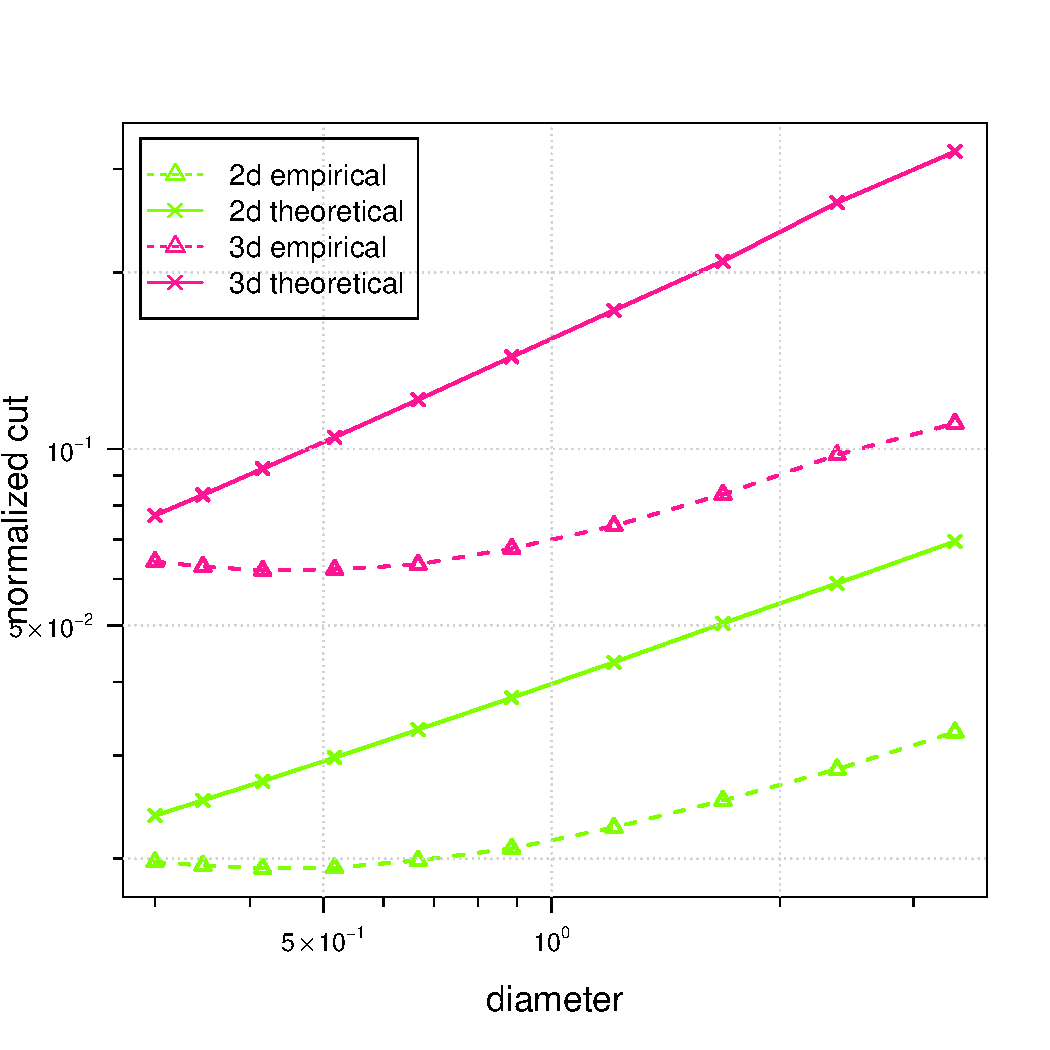
\includegraphics[width=\linewidth]{example1plots/diameter_normalized_cut_plot}
      \caption{}
    \end{subfigure}
    \begin{subfigure}{.33\linewidth}
      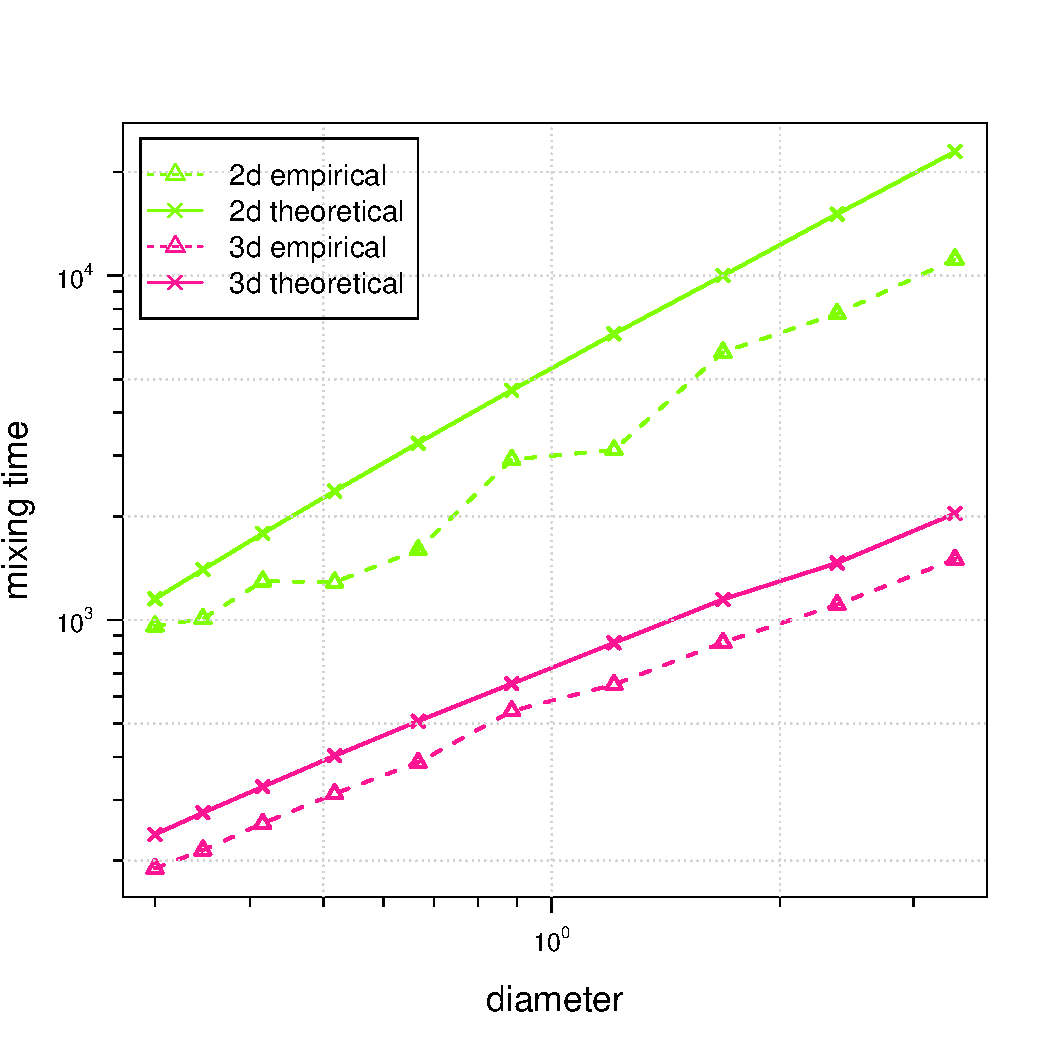
\includegraphics[width=\linewidth]{example1plots/diameter_mixing_time_plot}
      \caption{}
    \end{subfigure}
    \caption{Samples, empirical results, and theoretical bounds for mixing time
      and normalized cut as diameter and thickness are varied. In (a) and (b),
      points in $\Cset$ are colored in red; points in $\Csig \setminus \Cset$
      are colored in yellow; and remaining points in blue.} 
    \label{fig:fig1}
  \end{adjustbox}
\end{figure}

As we do not provide any theoretical lower bounds, we investigate the tightness of Theorems \ref{thm: conductance_upper_bound} and \ref{thm: mixing_time_upper_bound} via simulation. Figure \ref{fig:fig1} compares these theoretical bounds with the empirical quantities \eqref{eqn: normalized_cut} and \eqref{eqn: mixing_time}, as we vary the diameter $\rho$ and thickness $\sigma$ of a cluster $\Cset$. Panels $(a)$ and $(b)$ show the resulting empirical clusters for two different values of $\rho$ and $\sigma$.

Panels $(d)$ and $(f)$ show our theoretical bounds on mixing time tracking closely with empirical mixing time, in both 2 and 3 dimensions.\footnote{Note that we have rescaled all values of theoretical upper bounds by a constant, in order to mask the effect of large universal constants in these bounds. Therefore only comparison of slopes, rather than intercepts, is meaningful.} This provides empirical evidence that the upper bound on mixing time given by Theorem \ref{thm: mixing_time_upper_bound} has the right dependency on both expansion parameter $\sigma$ and diameter $\rho$. The story in panels $(c)$ and $(e)$ is less obvious. We note that while, broadly speaking, the trends do not appear to match, this gap between theory and empirical results seems largest when $\sigma $ and $\rho$ are approximately equal. As the ratio $\rho/\sigma$ grows, we see the slopes of the empirical curves become more similar to those predicted by theory.

\paragraph{Empirical behavior of \ppr}

\begin{figure}
	\centering
	\begin{adjustbox}{minipage=\linewidth}
		\begin{subfigure}{.24\linewidth}
			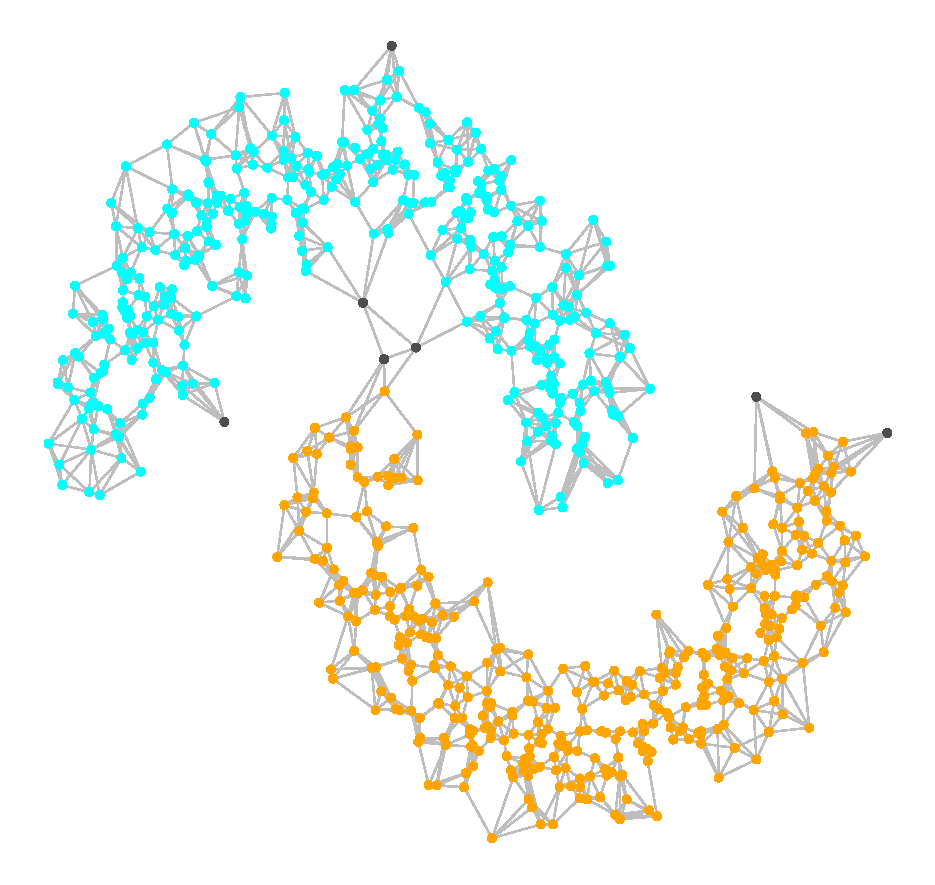
\includegraphics[width=\linewidth,scale = .5]{example2plots/row1_true_density_cluster}
			\caption{}
		\end{subfigure}
		\begin{subfigure}{.24\linewidth}
			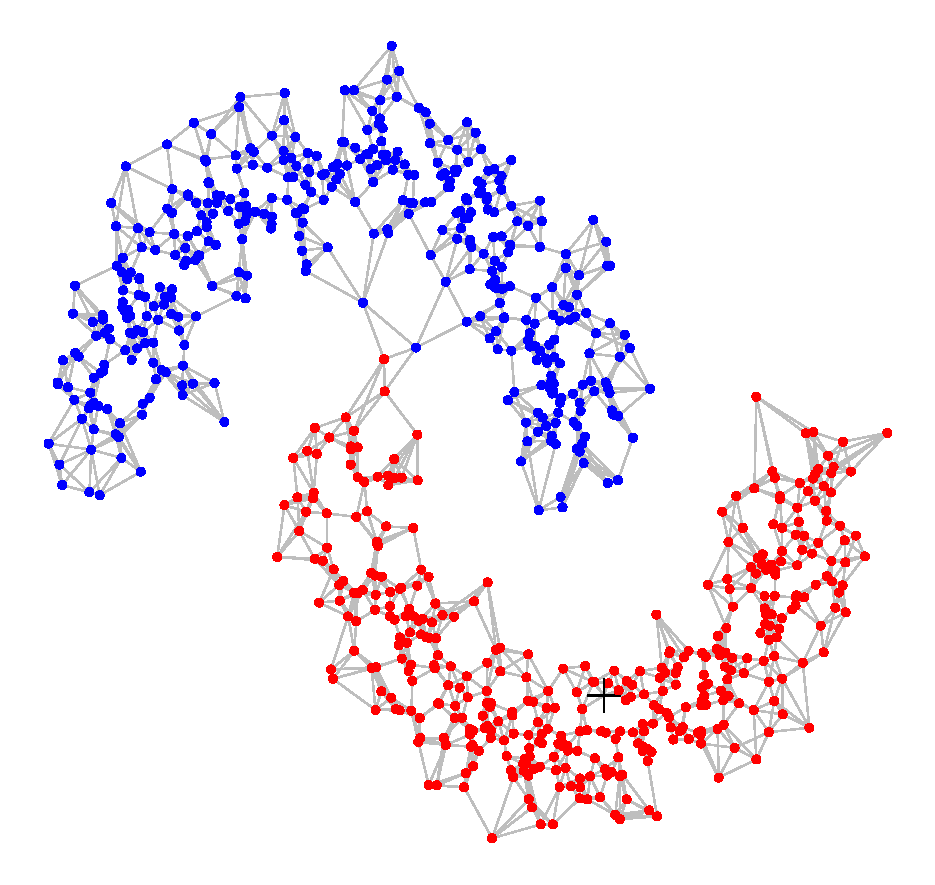
\includegraphics[width=\linewidth]{example2plots/row1_ppr_cluster}
			\caption{}
		\end{subfigure}
		\begin{subfigure}{.24\linewidth}
			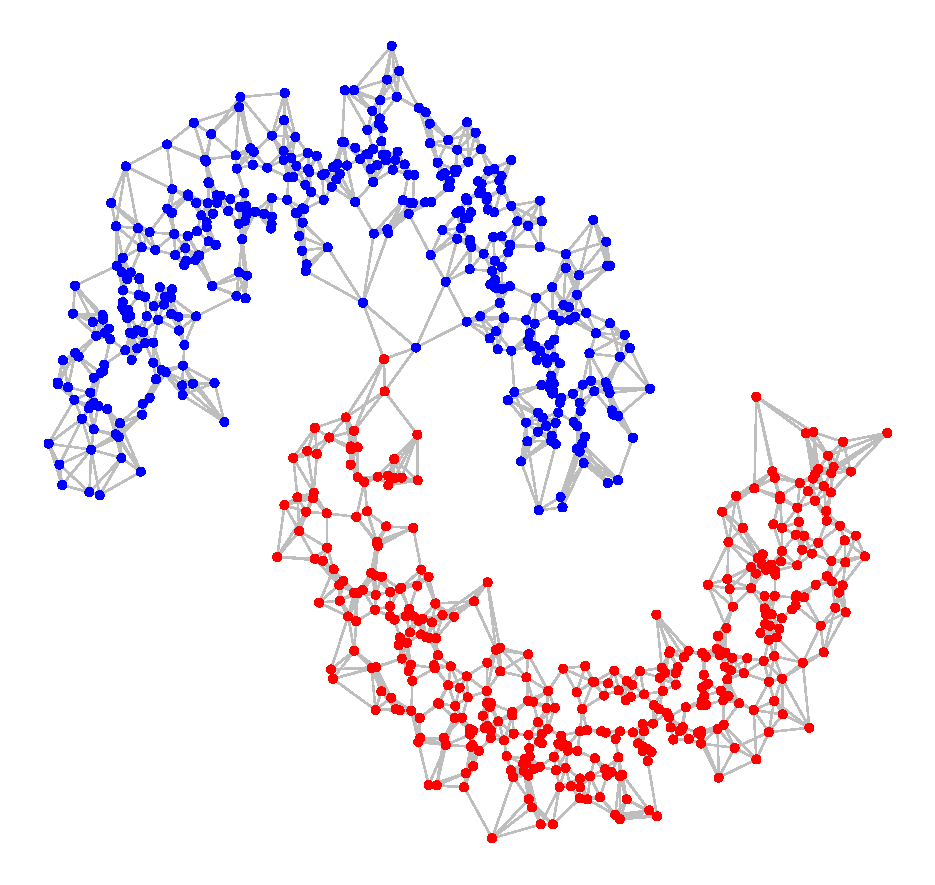
\includegraphics[width=\linewidth]{example2plots/row1_conductance_cluster}
			\caption{}
		\end{subfigure}
		\begin{subfigure}{.24\linewidth}
			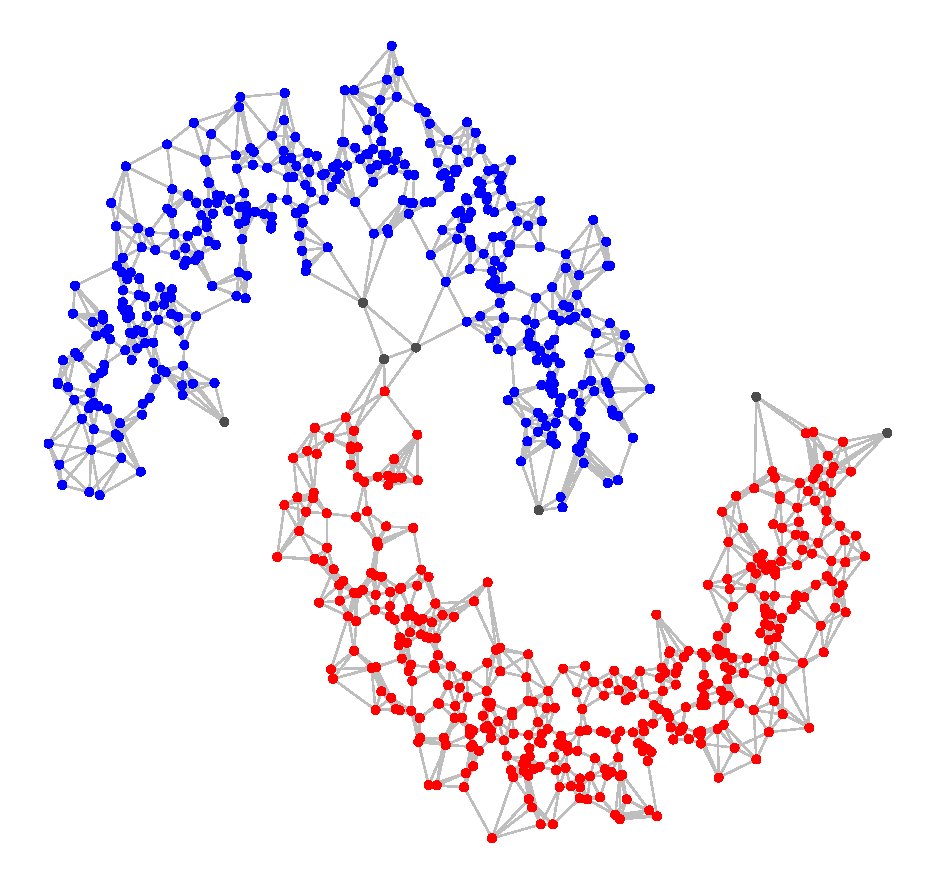
\includegraphics[width=\linewidth]{example2plots/row1_density_cluster}
			\caption{}
		\end{subfigure}
		
		\begin{subfigure}{.24\linewidth}
			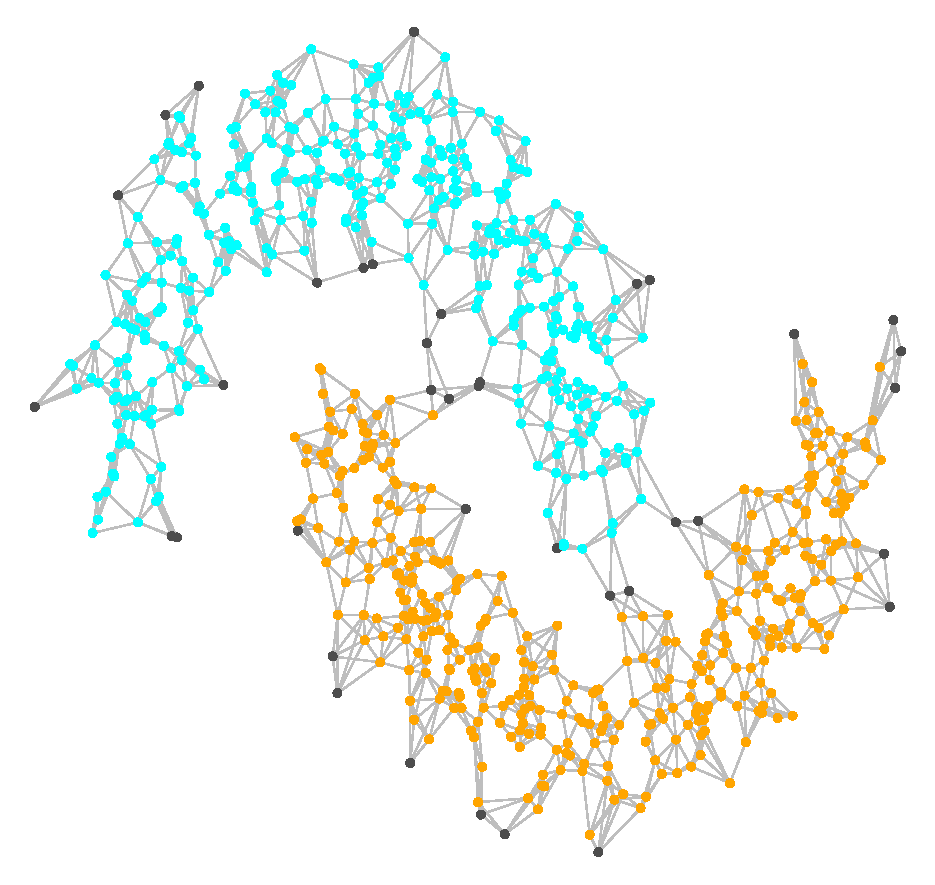
\includegraphics[width=\linewidth]{example2plots/row2_true_density_cluster}
			\caption{}
		\end{subfigure}
		\begin{subfigure}{.24\linewidth}
			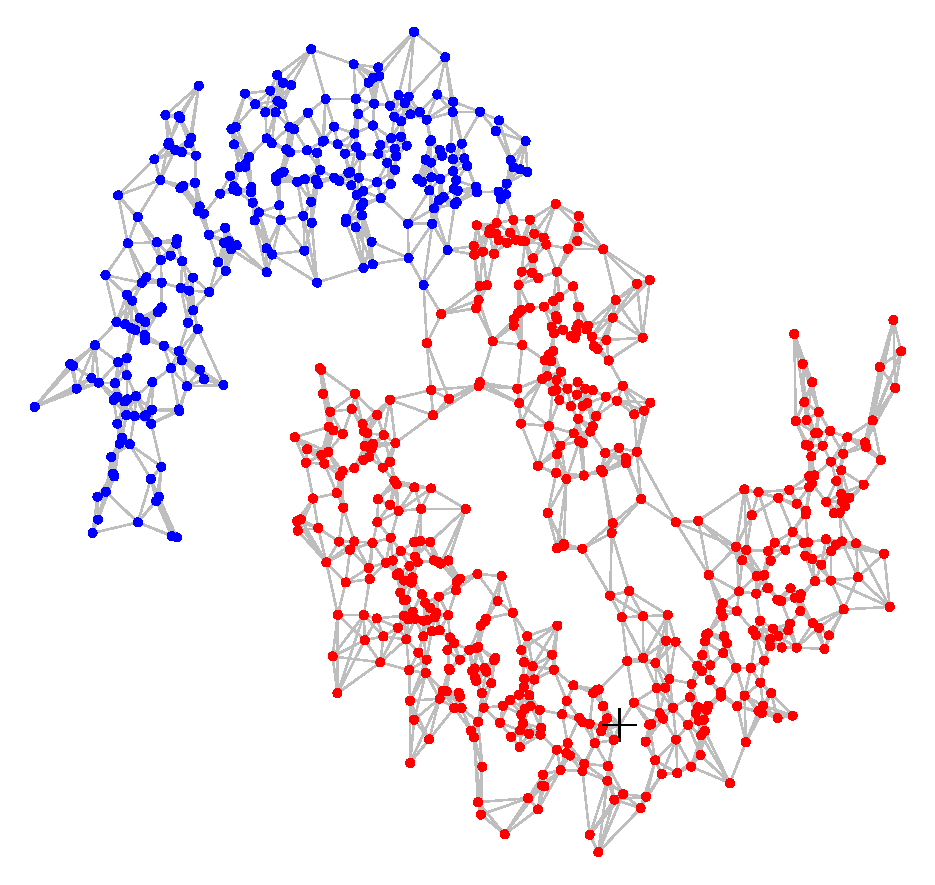
\includegraphics[width=\linewidth]{example2plots/row2_ppr_cluster}
			\caption{}
		\end{subfigure}
		\begin{subfigure}{.24\linewidth}
			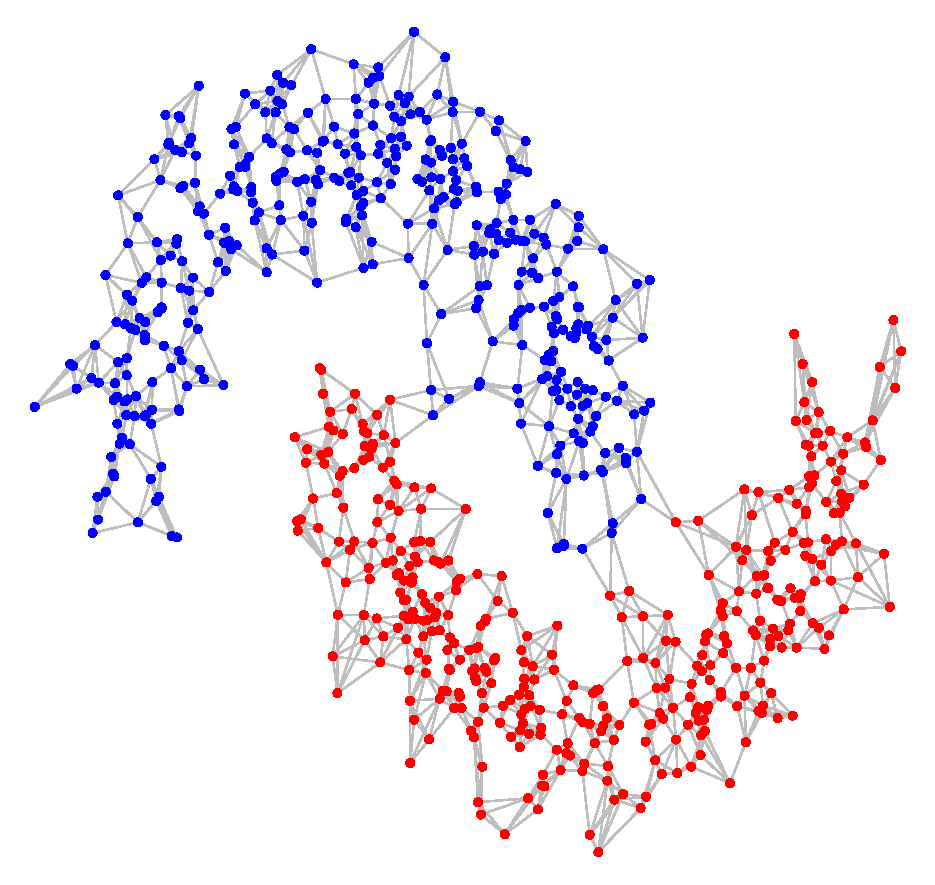
\includegraphics[width=\linewidth]{example2plots/row2_conductance_cluster}
			\caption{}
		\end{subfigure}
		\begin{subfigure}{.24\linewidth}
			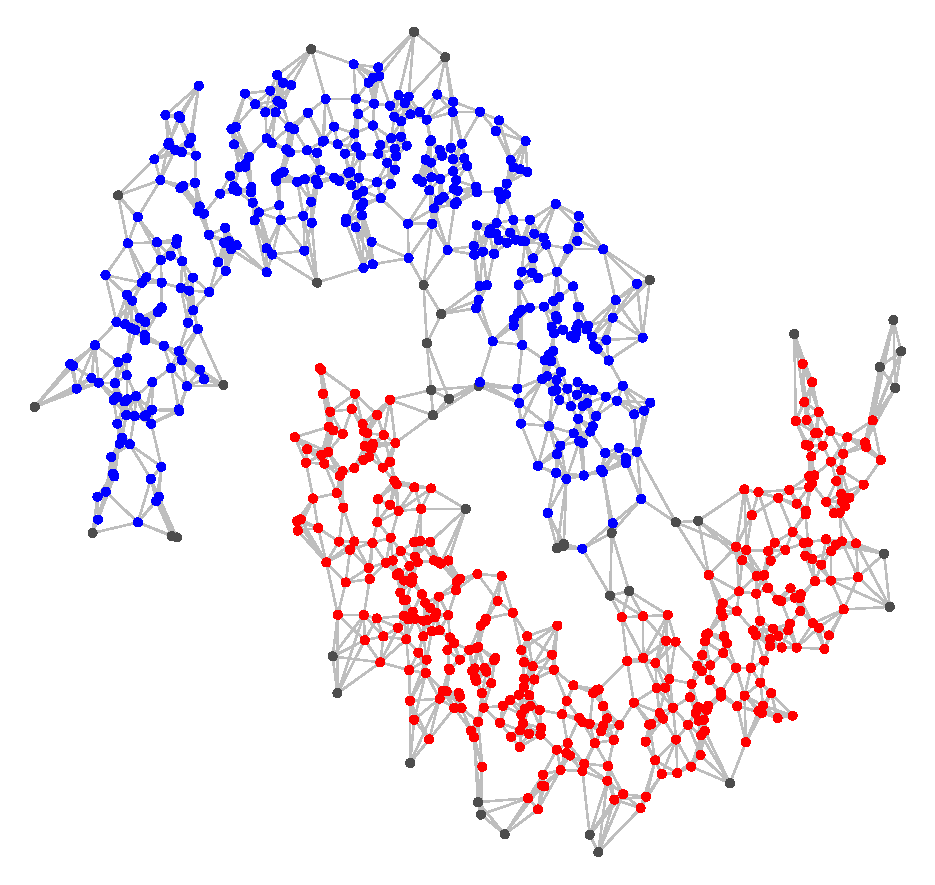
\includegraphics[width=\linewidth]{example2plots/row2_density_cluster}
			\caption{}
		\end{subfigure}
		
		\begin{subfigure}{.24\linewidth}
			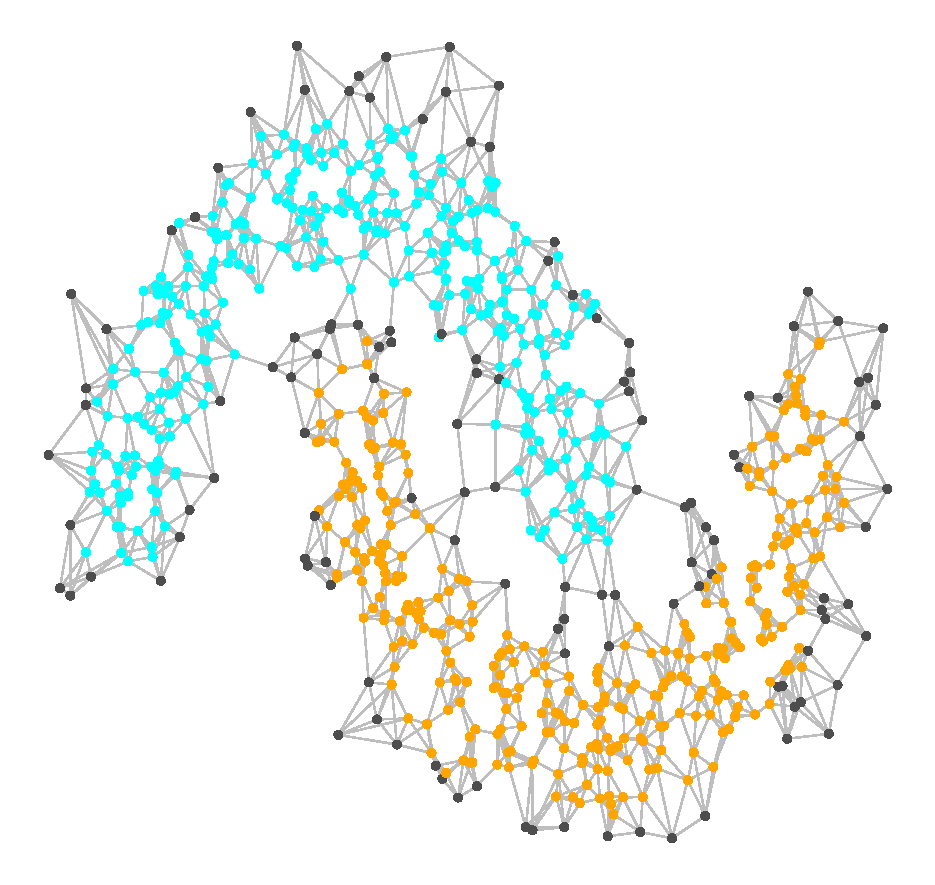
\includegraphics[width=\linewidth]{example2plots/row3_true_density_cluster}
			\caption{}
		\end{subfigure}
		\begin{subfigure}{.24\linewidth}
			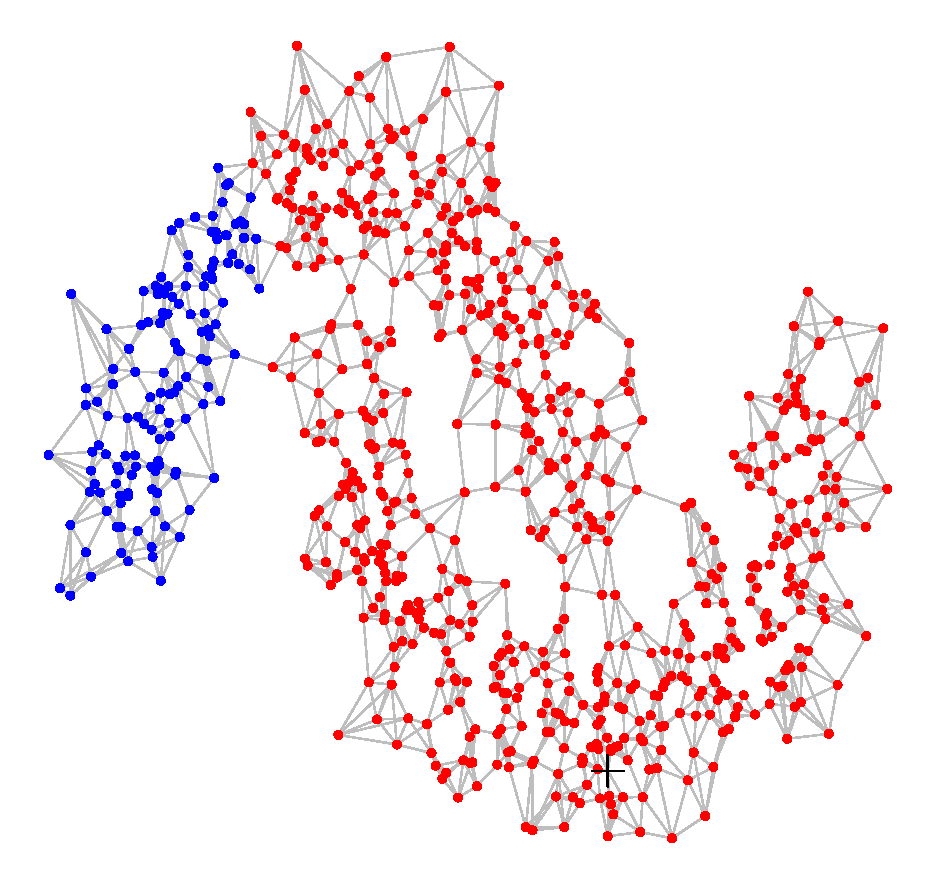
\includegraphics[width=\linewidth]{example2plots/row3_ppr_cluster}
			\caption{}
		\end{subfigure}
		\begin{subfigure}{.24\linewidth}
			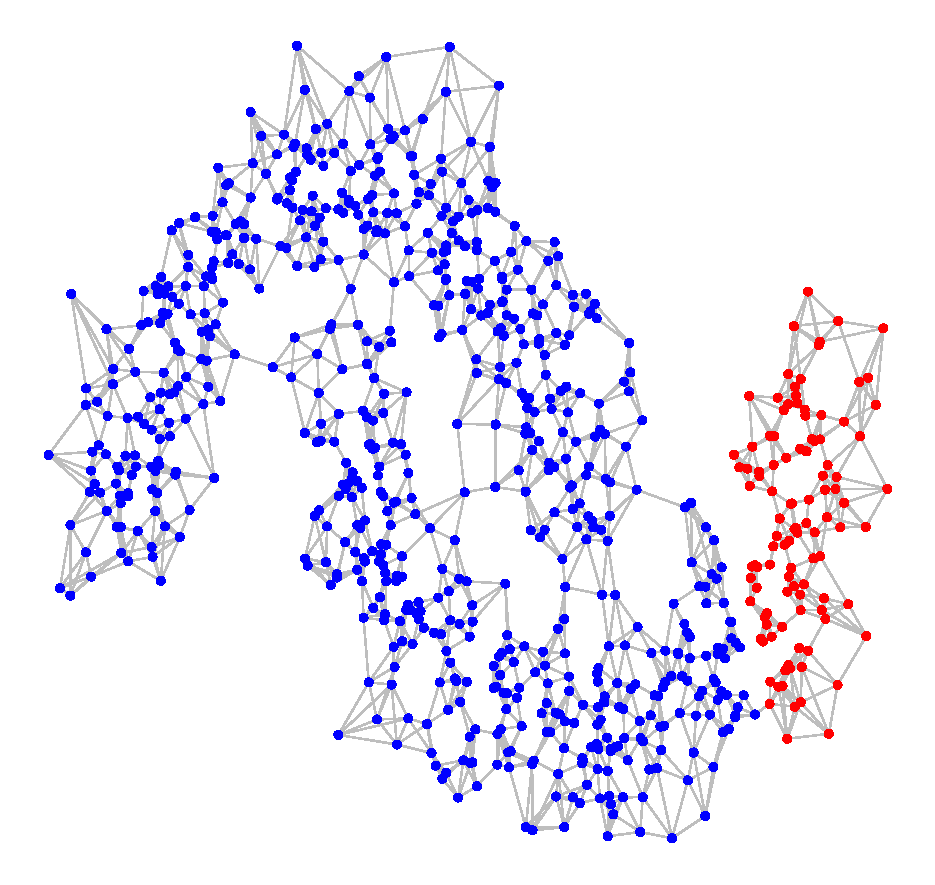
\includegraphics[width=\linewidth]{example2plots/row3_conductance_cluster}
			\caption{}
		\end{subfigure}
		\begin{subfigure}{.24\linewidth}
			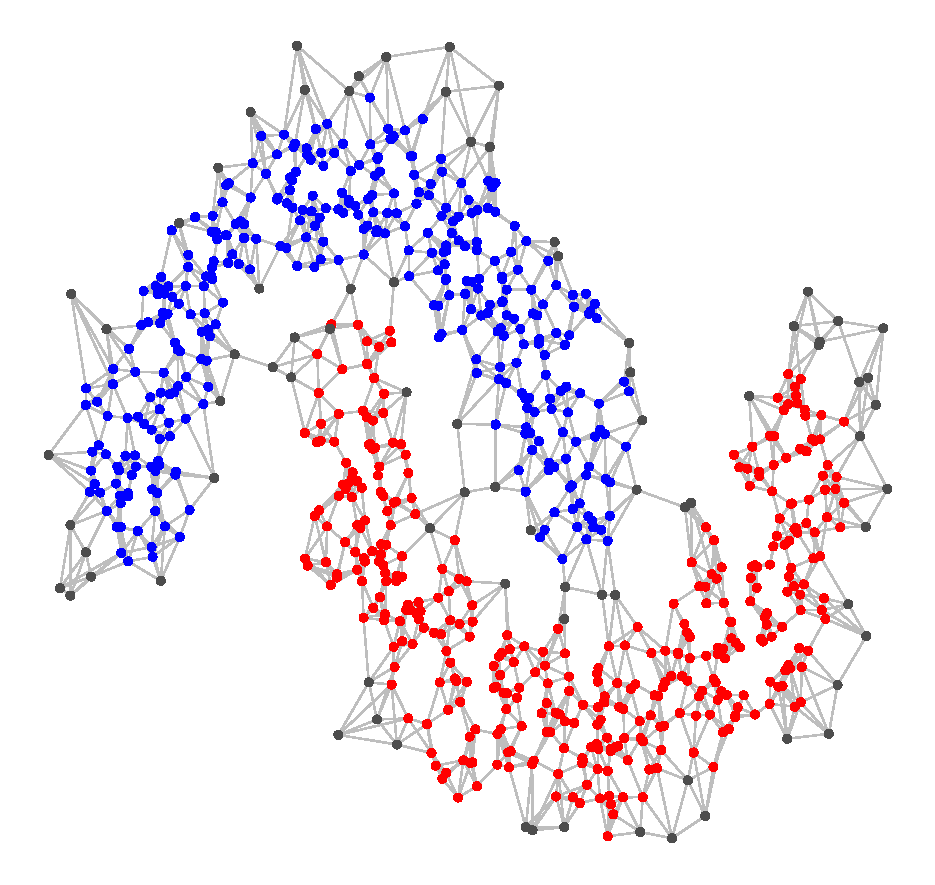
\includegraphics[width=\linewidth]{example2plots/row3_density_cluster}
			\caption{}
		\end{subfigure}
		\caption{True density (column 1), \pprspace (column 2), normalized cut (column 3) and estimated density (column 4) clusters for 3 different simulated data sets. Seed node for \pprspace denoted by a black cross.}
		\label{fig:fig2}
	\end{adjustbox}
\end{figure}

To drive home the main implications of Theorems \ref{thm: misclassification_rate} and \ref{thm: consistent_recovery_of_density_clusters}, in Figure \ref{fig:fig2} we show the behavior of \ppr, normalized cut, and the density clustering algorithm of \citep{chaudhuri2010} on the well known ``two moons'' dataset (with added 2d Gaussian noise), considered a prototypical success story for spectral clustering algorithms. The first column consists of the empirical density clusters $C_n$ and $C_n'$ for a particular threshold $\lambda$ of the density function; the second column shows the cluster recovered by \ppr; the third column shows the global minimum normalized cut, computed according to the algorithm of \cite{szlam2010}; and the last column shows a cut of the density cluster tree estimator of \citep{chaudhuri2010}.

Figure \ref{fig:fig2} shows the degrading ability of \pprspace to recover density clusters as the two moons become less well-separated. Of particular interest is the fact that \pprspace fails to recover one of the moons even when normalized cut still succeeds in doing so, supporting our claim from Remark \ref{rmk: diameter}. Additionally, we note that a density clustering algorithm recovers a moon even when both \pprspace and normalized cut fail, lending empirical weight to our overall message that \pprspace recovers only geometrically well-conditioned density clusters.

\section{Discussion}
\label{sec: discussion}
For given data, there are an almost limitless number of ways to define what the ``right'' clustering is. We have considered one such notion -- density upper level sets -- and have detailed a set of natural geometric criteria which, when appropriately satisfied, translate to provable bounds on estimation of the cluster by \ppr. We do not, however, provide a theoretical lower bound showing that our geometric conditions are required for successful recovery on an upper level set. Although we investigate the matter empirically, this is a direction for future work.

\clearpage

\bibliographystyle{plainnat}
\bibliography{../local_spectral_bibliography}

\end{document}